\chapter{Caching Basics}
\label{chapter:caching-model}

In order to get a common understanding of caching and the terminology related to the topic, we will go through the basics of caching by describing the architecture of a web system using a cache, present a model based on a timeline that introduces the different events involved in caching and last we list criteria for evaluating a caching technique in order to choose an appropriate technique for a given use case.

\section{Basic Caching Algorithm}
\label{sec:caching_basics}

In general caching is about storing the result of a computation at a where you are able to retrieve it fast, such that it is possible to get the result fast instead of recomputing it. This basic algorithm is illustrated on figure~\ref{fig:basic-caching} and can be described as following:

\begin{figure*}[ht!]
  \centering
  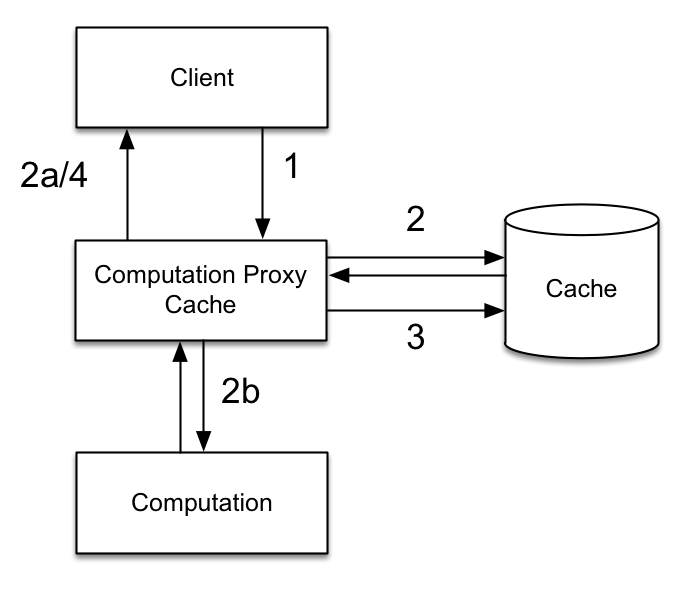
\includegraphics[width=0.6\linewidth]{figures/basic-caching-figure.pdf}
  \begin{enumerate}
    \item The result $v$ of a computation $f$ is requested.
    \item If $v$ is cached and is valid, we go to 5 with $v'=v$. Else we continue.
    \item We run the computation $f$
    \item The new result $v'$ of $f$ is stored in the cache.
    \item $v'$ is returned.
  \end{enumerate}
  \caption{The flow of basic caching}
  \label{fig:basic-caching}
\end{figure*}

In some cases, where the client is not allowed to wait for the computation to run, step 3-4 are replaced by a step that simply returns an empty value.

If we look at the cached object from an abstract point of view, we can see it as a \emph{result of a function} given certain \emph{inputs}. Sometimes the inputs are data from a storage system, sometimes it's the result of an API call to some external resource, sometimes it's global variables in the code. These \emph{inputs} we from now on be referred to as \emph{underlying data}.

% Also mention 'locality' here

In order for the algorithm to work, we need to be sure that when we store the cached object it has to be uniquely identified by some key such that when we lookup the value as in step 2 of the algorithm, we always locate $v$. This presents one of the challenges of cache management, which is in many cases closely related to cache invalidation (one of the two hard things in computer science\footnote{Not scientifically, but at least a favorite saying of Martin Fowler and quote by Phil Karlton}).

In the algorithm cache invalidation is simply described as a \emph{check}, but in reality this is the hard challenge of caching. The \emph{check} could be a precomputed indicator from earlier triggers, it could be based on a key derived from the underlying data or some timestamp. These cache invalidation approaches will be described more in section~\ref{sec:invalidation_techniques}.

\subsection{Architecture}
\label{subsec:architecture}

\begin{figure*}[ht!]
  \centering
  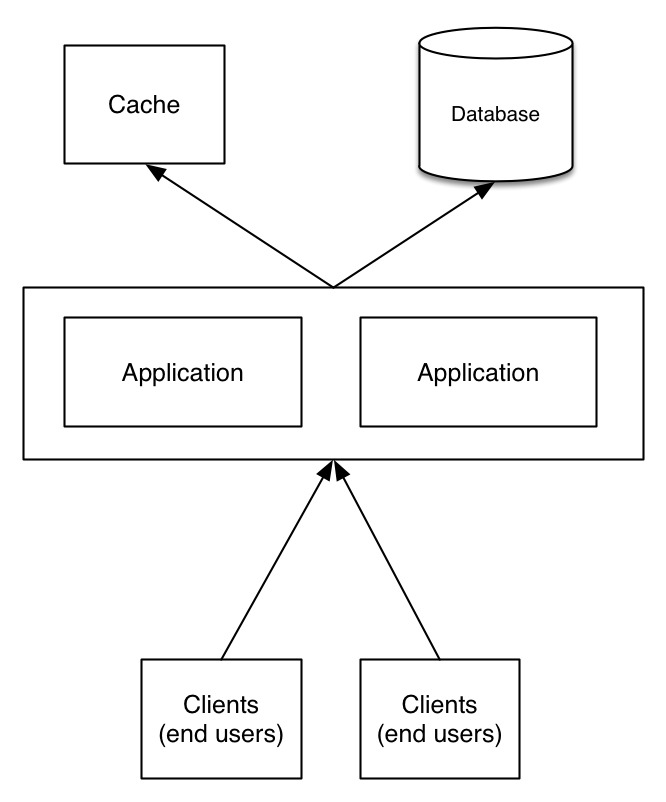
\includegraphics[width=0.5\linewidth]{figures/architecture.pdf}
  \caption{The assumed architecture of the system}
  \label{fig:caching-basics-architecture}
\end{figure*}

The architecture of the web application in which the cache is used is important to how the cache system. We assume that the architecture of the system is a common web application architecture as illustrated in figure~\ref{fig:caching-basics-architecture} consisting of a web application that serves HTTP-requests from the client (represented by the user) and interacts with a primary storage database to store and load data. To store and fetch the cached content we introduce a cache database. This could easily be the same unit as the primary storage database, but we separate them for better clarification.

Most modern web applications needs to serve multiple users at the same time, which means the web application must run on multiple processes\footnote{This is processes as an abstract term used in distributed systems. If we need to be implementation specific this could just as well be threads.} either on a single or multiple machines. We will therefore treat the web application as a distributed system.

A popular choice for cache databases are key-value stores such as Redis~\footnote{http://redis.io/} and Memcached~\footnote{https://memcached.org/} since they are simple distributed key-value stores that lives in memory and therefore allows for scalability and high-performance operations. In order to support most practical web applications, we will therefore make the assumption that the cache database has the same functionality: it should be possible to store arbitrary content for a given key. Furthermore the final solution of this thesis require the cache database to support atomic transactions for a given key, which are supported in Memcached using the CAS command~\cite{docs:memcached-protocol} and in Redis using the \verb$WATCH$-command~\cite{docs:redis-transactions}. The reasons behind this assumption will be explained more in chapter~\ref{chapter:data-update-propagation}.

\subsection{Cache Server}
\label{subsec:cache-server}

% subsection cache-server end

% subsection architecture end

\subsection{Timeline Model}
\label{subsec:timeline_model}

As with the algorithm on figure~\ref{fig:basic-caching}, caching can be described by a series of events. The ordering of events decides whether the cached content or a fresh computation is presented to the client. To describe the different caching techniques, we will use a timeline model with a stream of events. One timeline describes the events occurring in a single process. We can therefore assume that there exists a total ordering of events for a single timeline. To be able to describe the caching techniques explained in this thesis, we will define the following events:

\begin{itemize}
  \item \textbf{Requested} is the event occurring when a client requests a given cached object
  \item \textbf{Computation Started} is when the computations is started
  \item \textbf{Computation Finished} is when the computation is finished and a result is returned
  \item \textbf{Stored} is happening when a given cached object is stored in the cache database
  \item \textbf{UD Updated} is when the underlying data has been updated
  \item \textbf{Invalidated} is when the system has knowledge that the cached object is invalidated
\end{itemize}

Alongside these events the timeline model illustrates the interval in which the given cached object is considered valid (the cache system will serve the cached value) and when it is actually fresh (consistent with underlying data). The validity interval illustrates when the cache system will respond immediately, which means if the cached object is always considered valid then the approach supports immediate responses. In the time interval, where the fresh and valid interval overlaps, the approach will serve a fresh version of the cached value. If they always overlap then the given approach will guarantee strict freshness.

The timeline model applied to the basic caching algorithm~\ref{fig:basic-caching} is illustrated on figure~\ref{fig:basic-caching-timeline}.

\begin{figure*}[ht!]
  \centering
  \includegraphics[width=1.0\linewidth]{figures/timeline/basic-caching.pdf}
  \caption{The timeline model applied to the basic caching algorithm}
  \label{fig:basic-caching-timeline}
\end{figure*}

% subsection timeline_model end

% section caching_basics end

\section{Evaluating Caching Techniques}
\label{sec:evaluating_caching_techniques}

% Goals of caching

To choose the correct caching technique for a given use case, we need to know the criteria for finally picking the best suited. The overall goal of caching in web development is to achieve a better user experience by getting a better performance and to save money by using less CPU power. If we assume that the cache system is able to retrieve cached objects fast, the goals can be achieved by ``hitting the cache'' as often as possible. We can measure this using the metric \emph{cache hit rate}, which refers to the rate at which the cache is hit among the total number of requests for the cached object.

%% END CORRECTNESS

% Intro: from perspective of user

To evaluate the caching technique for a given use case, we will see the situation from the perspective of the client (i.e. a user). The client makes a request for some content that is served by the web server. This content contains of one or more computations that can be cached individually.

%%%% CONSISTENCY

We will not make any assumptions about the content send by the server, which means the content could be the result of multiple cached computations. Each of these computations are based on some underlying data e.g. served from the primary store. In the case where some computations are based on the same data we have to keep the different results consistent. Furthermore the response might be based on both cached content and content loaded directly from the primary store in which case we have to keep the data consistent across the cache database and the primary storage. This issue leads to the criteria keeping consistency between the data.

There exists multiple levels of consistency, but to keep it relevant and simple, we will evaluate the level of consistency using a binary value: either the caching technique ensures consistency with the data from the primary storage or else it doesn't.

%%%% FRESHNESS

Another parameter is the freshness of the content returned by the cache. It is most desirable to have content that is as fresh as possible as oppose to having stale data, but in the end the goal is to make the served content make sense for the user. Consider example~\ref{example:peergrade-split-interface} of the Peergrade.io platform, where there are two types of users. If the teacher changed the description of an assignment and a student requested and read the description 1 min after then it would not be unexpected behaviour to show the old description from the students point of view. On the other hand if the teacher requested the description 1 min after, it would be unexpected behaviour to show the teacher an old version, since the teacher would think the description hasn't been updated. We will represent freshness as a binary parameter that we call ``Strict Freshness'', which evaluates whether a given cached object that is fetched is guaranteed to be fresh.

\begin{example}
\label{example:peergrade-split-interface}
At Peergrade.io the web application has a teacher and a student interface. Teachers create assignments and sees statistics about the grades students have given to each other through their feedback. The students see the assignments created by their teachers, are able to hand in their assignments, and grade other students' hand in.
\end{example}


%%%% WAITING TIME AFTER INVALIDATION

While the freshness describes what is expected behaviour with relation to the content, there also exists time limits with relation to keeping the user focused on the task. Miller and Card et. al.~\cite{paper:miller-response-time-limit, paper:card-response-time-limit} describes these limits as:

\begin{itemize}
  \item When the response time is \textbf{0.1 second} the user feels that the system is \textbf{reacting instantaneously}.
  \item A response time above \textbf{1 second} will \textbf{interrupt the user's flow of thought}.
  \item \textbf{10 seconds} is limit related to \textbf{keeping the user's attention} on the given dialog.
\end{itemize}

In the basic caching algorithm described on figure~\ref{fig:basic-caching}, the computation has to run after it has been invalidated. If the caching technique runs this computation in the same process as the request from the client, the client has to wait for the computation to finish in order to show the content to the user. If the time taken to compute the value exceeds the accepted response time limits described above, it could become critical for the user experience. Based on this fact we will introduce the binary parameter of whether or not the client has to wait for the computation to finish after invalidation. The weight of this parameter is proportional to the cache miss rate since it's only requests, which results in a cache miss that are affected by the slow response time.

%%%% AUTOMATIC UPDATE/INVALIDATION

It is not possible to both serve the cached objects immediately and have strict freshness. This can be proved using the example where a cached object is invalidated just before it is requested. We can only start computing the value at the moment it has been invalidated and given that the time between the invalidation and the request is smaller than the time taken to compute the value, it is not possible.

In cases where we choose immediate response time and we can tolerate serving cached objects that are not strictly fresh, we might want to keep the cached objects as up to date as possible. This means that we start computing the cached objects as soon as they have been invalidated. In order to achieve this we need some mechanism that invalidates depending cached objects when underlying data are updated. We will also represent ``Automatic Invalidation'' as a binary parameter.

%%%% CACHE MANAGEMENT

So far we've considered parameters from a user's perspective, but to evaluate the caching technique fully we also need to see it from the perspective of the programmer since a big part of cache management is manually tracking dependencies between the cached content and the underlying data. We want the caching system to be transparent such that it is easy to add and remove caching from existing computations. Additionally we want the caching system to be robust such that when new code involving a cached computation is added, it should behave as expected without introducing errors. We cannot measure the level of robustness so we will therefore introduce the binary criteria: does the caching technique involve maintenance with relation to invalidation (shortened as invalidation maintenance)?

%%%% ADAPTABILITY

The last parameter we will introduce is also a requirement of the system: \emph{adaptability}. Since adaptability cannot be evaluated objectively we will introduce a scale of \emph{high}, \emph{medium} and \emph{low}, where high means that is adaptable to most systems and low means that it is adaptable to a few systems. We will define the scale as following:

\begin{itemize}
  \item \textbf{Low}: The technique has assumptions about the primary data store, cache database and/or application that means it cannot be applied to other common technologies.
  \item \textbf{Medium}: The technique is advanced and requires a lot of implementation effort or external libraries/processes to work.
  \item \textbf{Low}: The technique can easily be implemented and applied to existing applications.
\end{itemize}

The reason behind the \emph{Low} criteria is that when the technique has assumptions about the technology behind the application it means the system is tied to using specific technologies, which makes it difficult to change when the given technology is obsolete or the requirements of the system change. If this is not considered a problem \emph{Low} and \emph{Medium} can be considered the same level of adaptability.

From this discussion, we can sum up the evaluation parameters as follows:

\begin{itemize}
  \item \textbf{Consistency}: The cached object must be consistent with the data from the primary storage
  \item \textbf{Strict Freshness}: The cached object must be as fresh as the state of the primary store when the value was requested
  \item \textbf{Automatic Update}: The cached object is automatically updated after it has been invalidated
  \item \textbf{Always Immediate Response}: The cached object must be served immediately after it has been requested
  \item \textbf{Invalidation Management}: Whether the programmer has the responsibility of maintaining the invalidation of the cached objects
  \item \textbf{Adaptability}: How adaptable the caching technique is to existing systems
\end{itemize}

% chapter caching_model end

